\documentclass[prb]{revtex4-2}
\usepackage{braket,amsmath,amssymb,color,graphicx,hyperref}
\begin{document}
\title{Wavefunction evolution under the unitary renormalisation group method}

\maketitle

\section{General idea behind a reverse URG analysis}
A reverse URG analysis involves studying the evolution of wavefunctions from the IR to the UV, by implementing inverse renormalisation group transformations. This is made possible by the fact that the IR fixed point Hamiltonians are often tractable and allow the computation of wavefunctions. Such an analysis gives insight into how states change as high-energy quantum fluctuations are resolved during the Hamiltonian renormalisation from the UV to the IR. It also allows studying the evolution of entanglement measures and correlation functions.

We will start with a very simple IR ground state wavefunction, and then go back towards the UV ground state by applying the inverse unitary operator \(U^\dagger\):
\begin{equation*}\begin{aligned}
	U : \underbrace{\ket{1,2,...,N}}_\text{UV ground state} \rightarrow \ket{1,2,...,N-1}\ket{N} \rightarrow ... \rightarrow \underbrace{\ket{1,2,...,N^*}\ket{N^*+1}...\ket{N}}_\text{IR ground state}
\end{aligned}\end{equation*}
\begin{equation*}\begin{aligned}
	U^\dagger : \underbrace{\ket{1,2,...,N^*}\ket{N^*+1}...\ket{N}}_\text{IR ground state} \rightarrow \ket{1,2,...,N^*+1}\ket{N^*+2}...\ket{N} \rightarrow ... \rightarrow\underbrace{\ket{1,,2,...,N}}_\text{UV ground state}
\end{aligned}\end{equation*}
The first process is the forward RG which we used to obtain the scaling equations.
The second process is the reverse RG which we will undertake now. The method has already been applied to study the renormalisation of entanglement in various models of strong correlation.
In general, we start with an IR wavefunction that consists a certain number of momentum states \(n_1\) still entangled with the impurity, and the remaining momentum states \(n_2\) disentangled from the impurity.
The former are said to be part of the emergent Kondo cloud, while the latter are said to be part of the integrals of motion (IOMs) and appear in direct product with the cloud+impurity system in the ground state wavefunction.
Each momentum state is tagged with two conduction bath levels, one above the Fermi surface and one below.
These will be represented as \(k,\pm\). If we represent the emergent cloud momentum states as \(\left\{k_i\right\} \) and the IOM states as \(\left\{q_i\right\}\), the ground state wavefunction can be written as 
\begin{equation}\begin{aligned}
	\ket{\Psi}_0 = \left(\otimes_{i=1}^{n_2}\ket{q_i,-,\uparrow}\ket{q_i,-,\downarrow}\right)\ket{\Phi}_\text{cloud}\left(\otimes_{i=1}^{n_2}\ket{q_i,+,\uparrow}\ket{q_i,+,\downarrow}\right)
\end{aligned}\end{equation}
Throughout, we have assumed that the IOMs below the Fermi surface are occupied while those above are unoccupied. This means:
\begin{equation}\begin{aligned}
	\ket{\Psi}_0 = \left(\otimes_{i=1}^{n_2}\ket{\hat n_{q_i,-,\uparrow}=1}\ket{\hat n_{q_i,-,\downarrow}=1}\right)\ket{\Phi}_\text{cloud}\left(\otimes_{i=1}^{n_2}\ket{\hat n_{q_i,+,\uparrow}=0}\ket{\hat n_{q_i,+,\downarrow}=0}\right)
\end{aligned}\end{equation}
\(\ket{\Phi}_\text{cloud}\) will be obtained by diagonalising a small system of \(n_1\) conduction bath \(k\) states. This completes the construction of the IR ground state \(\ket{\Psi}_0\). The algorithm of reverse RG then involves applying unitary transformations on this IR wavefunction; the unitary transformations will be the inverse of those that were applied during the forward RG algorithm. Since the forwards RG transformations decoupled \(k\) states and transformed them into the IOMS, the inverse transformations will take the momentum states in the IOMs and re-entangle them with the impurity+cloud system, one at a time. This is shown in fig.~\ref{rev-rg}.
\begin{figure}[!htbp]
	\centering
	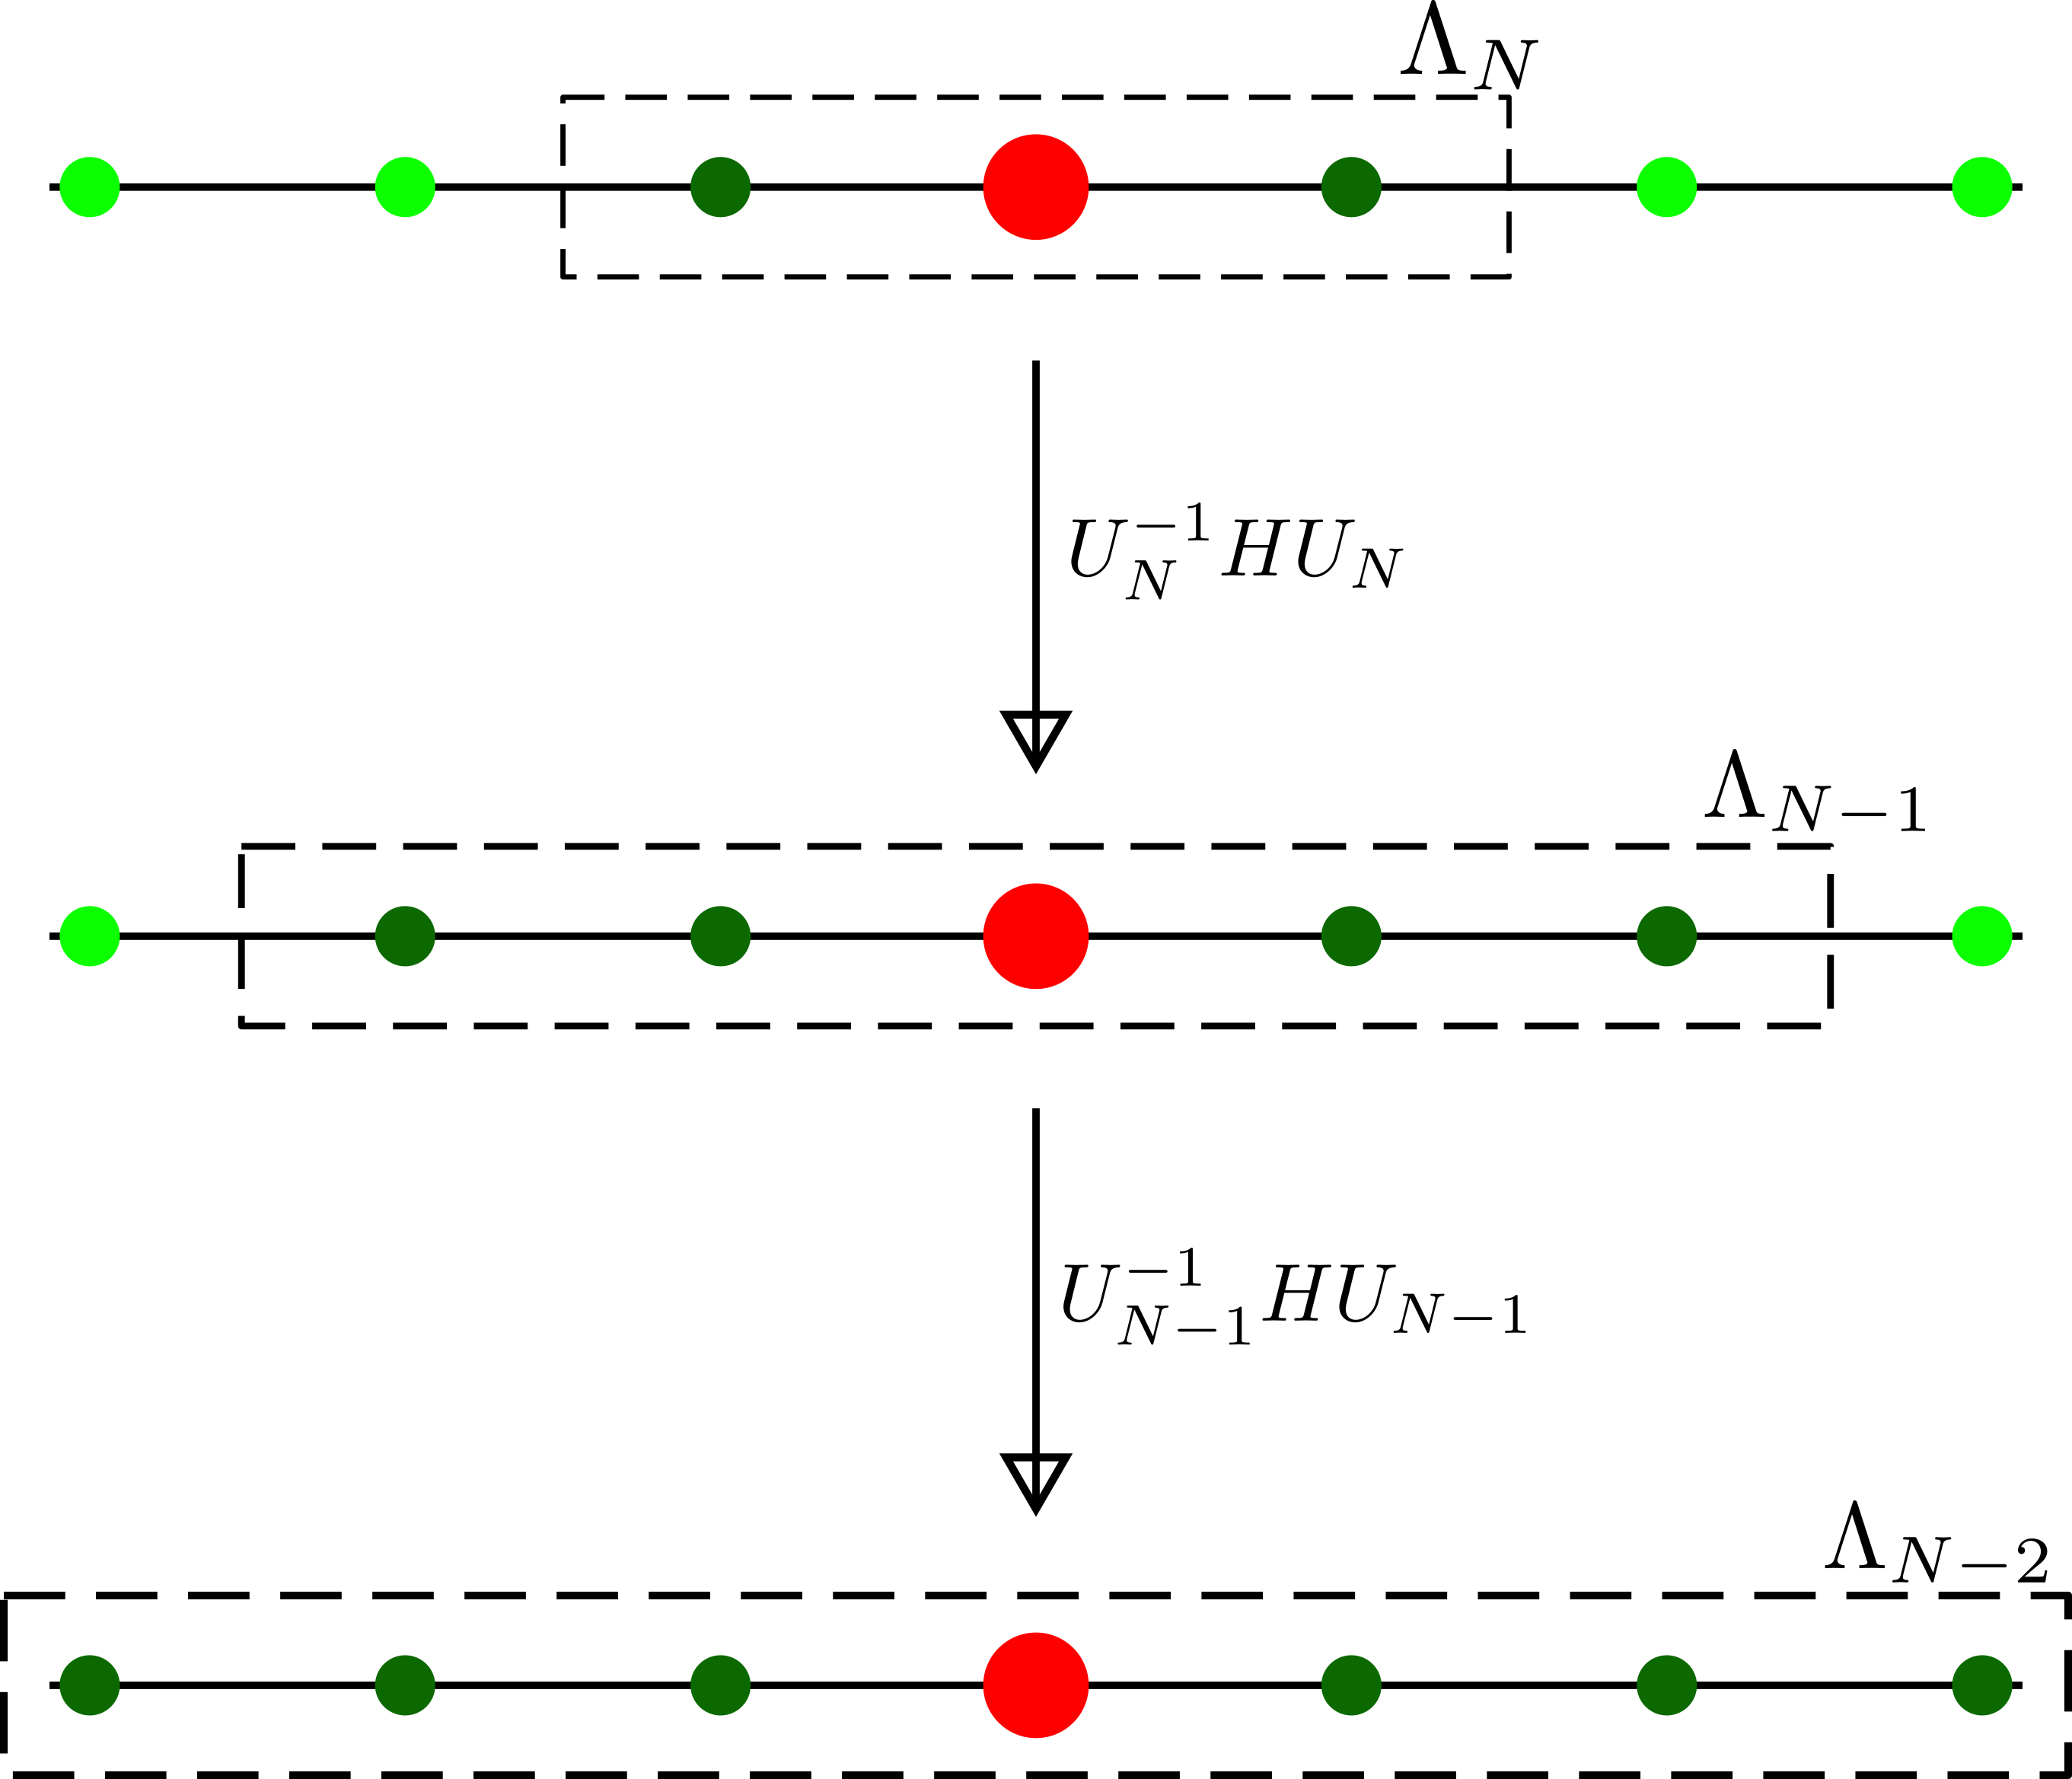
\includegraphics[width=0.4\textwidth]{reverse-rg.png}
	\caption{We start with a Hamiltonian with an impurity site (red) coupled with two conduction electrons (dark green), with four other decoupled electrons (bright green). The dotted rectangle represents the emergent window \(\left( -\Lambda_j, \Lambda_j \right) \) at each step; the electrons inside that rectangle are still entangled with the impurity, while the ones inside have been decoupled. The next step of reverse RG involves applying the inverse transformation on the Hamiltonian, which will couple two more electrons from the IOMS (hence four dark green circles in the second step), leading to an enlargement of the emergent window. The unitary varies for each step, hence the notation \(U_j\).}
	\label{rev-rg}
\end{figure}

The next step is to write down the unitaries that will take us from the IR ground state to the UV ground state. In the forward RG, we used the following unitary for decoupling the shell \(\epsilon_q\) and spin \(\beta\) is
\begin{equation}\begin{aligned}
	U_{q\beta} = \frac{1}{\sqrt 2}\left[1 + \eta_{0 \beta} + \eta_{1\beta}^\dagger\right]~.
\end{aligned}\end{equation}
Here, the subscripts \(0\) and \(1\) indicate it decouples an electron above and below the Fermi surface respectively. The inverse transformation for re-entangling \(q\beta\) is
\begin{equation}\begin{aligned}
	U^\dagger_{q\beta} = \frac{1}{\sqrt 2}\left[1 + \eta_{0 \beta}^\dagger + \eta_{1\beta}\right]~.
\end{aligned}\end{equation}

The wavefunction after reversing one step of the RG will thus be
\begin{equation}\begin{aligned}
	\ket{\Psi}_1 = U^\dagger_{q \uparrow}U^\dagger_{q \downarrow}\ket{\Psi}_0
\end{aligned}\end{equation}
Here, \(q\) is the first momentum state immediately outside the emergent cloud. Re-entangling further momentum states using their respective unitaries lead to the sequence of wavefunctions \(\ket{\Psi}_2, \ket{\Psi}_3\) and so on.
A straightforward way of calculating entanglement and correlations across the RG flow is to create a second-quantised prototypical form of the IR state \(\ket{\Psi_0}\), and then apply the inverse unitary operators \(\left\{ U_i \right\} \) to this wavefunction in order to generate the family of states \(\ket{\Psi_i} = U_i \ket{\Psi_{i-1}}, i > 0\). Quantities like entanglement entropy and correlations can then be calculated by using this family of kets. Such a method, however, soon runs into problems of time complexity and physical memory usage. This is primarily because the operators and the kets are many-body in nature and grow exponentially in size as the number of electronic states are increased.

\section{Evolution equation for tensor network coefficients}
We will now show a more efficient method of computing quantities along the reverse RG operations. We will demonstrate this for the much simpler single-channel Kondo problem (which can be obtained from our model by setting all interactions apart from the Kondo coupling \(J\) to zero). For this, we will first have to perform some analytical groundwork. The URG transition operators for re-entangling the states at momentum \(q\) take the form
\begin{equation}\begin{aligned}
	\eta_{q\beta}^\dagger = \alpha(q)\sum_{k} \left( S_d^z \beta c^\dagger_{q\beta}c_{k\beta} + c^\dagger_{d\overline\beta}c_{d\beta}c^\dagger_{q\beta}c_{k\overline\beta}\right) ~,\\
	\eta_{q\beta} = \alpha(q)\sum_{k} \left( S_d^z \beta c^\dagger_{k\beta}c_{q\beta} + c^\dagger_{d\beta}c_{d\overline\beta}c^\dagger_{k\overline\beta}c_{q\beta}\right)~,
\end{aligned}\end{equation}
for the Kondo problem, where we have defined \(\alpha(q) = \frac{1}{d_2}\frac{J}{2}\). Let \((m_l)\) \(n_l\) be the number of momentum states that are (not) entangled with the impurity at the \(l^\text{th}\) step. The total dimension of the system is then \(N_l = 1 + 2m_l + 2n_l\), where \(1\) takes care of the impurity spin and the factors of 2 account for the spin degeneracy. We can write the groundstate at this step in the form
\begin{equation}\begin{aligned}
	\ket{\Psi}_l = \sum_{j=1}^{2^{N_l}} \mathcal{C}_l(s_j)\ket{\sigma^z_d=s_j(d)}\otimes_{i=1}^{m_l}\ket{n_{k_i}=s_j(k_i) }\otimes_{i=1}^{n_l}\ket{n_{q_i}=s_j(q_i)}\label{tensordecomposition}
\end{aligned}\end{equation}
where \(\left\{ s_j; j=0,\ldots,2^{N_l}-1\right\} \) is the Cartesian product of the set of occupancies \(\left\{ 0,1 \right\} \) of the \(N_l\) members, and the sum is over all the possible classical number conserved configurations. \(s_j(k_i)\) represents the occupancy (either 0 or 1) of the member \(k_i\) within the configuration \(s_j\). As an example, the configuration \(s_j = 1001\) means that the impurity spin has spin up \(\left( s_j(0) = 1 \right) \), the first and second momentum states are unoccupied \(\left( s_j(1) = s_j(2) = 0 \right) \) and the third momentum state is occupied \(\left( s_j(3) = 1 \right) \). Note that within the summation of eq.~\ref{tensordecomposition}, each momentum state also has a spin index which has been suppressed.

We will now apply the URG transition operators on such a general state. As a matter of bookkeeping, we will retain the configurations of states only up to the momentum index that will be decoupled at the current step, because the IOM states beyond it will not be modified at the current iteration.
\begin{equation}\begin{aligned}
	\eta_{q\beta} \ket{\Psi}_l = \sum_{j=1}^{2^{N_l}} \mathcal{C}_l(s_j) \alpha(q)\sum_{k} \left( S_d^z \beta c^\dagger_{k\beta}c_{q\beta} + c^\dagger_{d\beta}c_{d\overline\beta}c^\dagger_{k\overline\beta}c_{q\beta}\right) \ket{\sigma^z_d=s_j(d)}\otimes_{i=1}^{m_l}\otimes_{\beta}\ket{n_{k_i\beta}=s_j(k_i\beta) }\otimes_{\beta}\ket{n_{q\beta}=s_j(q\beta)}
\end{aligned}\end{equation}
where \(\beta = \pm 1\) runs over the spin indices. Note that the first part of the transition operator only picks out classical configurations that satisfy \(n_{k\beta} = 1 - n_{q\beta} = 0\). Similarly, the second part picks out configurations with \(n_{k\bar\beta} = 1 - n_{q\beta} = 0, \sigma_d^z = \bar\beta\). The expression therefore evaluates to 
\begin{equation}\begin{aligned}
	\eta_{q\beta} \ket{\Psi}_l = \sum_{j=1}^{2^{N_l}} \mathcal{C}_l(s_j) \alpha(q)\sum_{k} \left[ \delta_{s_j(k\beta),0}\delta_{s_j(q\beta),1} S_d^z \beta c^\dagger_{k\beta}c_{q\beta} \ket{\sigma^z_d=s_j(d)}\otimes_{i=1}^{m_l}\otimes_{\beta}\ket{n_{k_i\beta}=s_j(k_i\beta) }\otimes_{\beta}\ket{n_{q\beta}=s_j(q\beta)} \right.\\
	\left.+ \delta_{s_j(d),(1 - \bar\beta)/2}\delta_{s_j(k\bar\beta),0}\delta_{s_j(q\beta),1}c^\dagger_{d\beta}c_{d\overline\beta}c^\dagger_{k\overline\beta}c_{q\beta} \ket{\sigma^z_d=s_j(d)}\otimes_{i=1}^{m_l}\otimes_{\beta}\ket{n_{k_i\beta}=s_j(k_i\beta) }\otimes_{\beta}\ket{n_{q\beta}=s_j(q\beta)}\right]
\end{aligned}\end{equation}
The first Kronecker delta in the second term, \(\delta_{s_j(d),(1 + \beta)/2}\), ensures that \(s_j(0)\) is unity when \(\beta = -1\) and zero when \(\beta = 1\). We can now apply the fermionic and spin operators on the states. We first consider the spin-preserving operator \(c^\dagger_{k \beta}c_{q \beta}\), and apply it on the ket, paying attention to any sign changes arising from fermion exchanges. Since the pair itself is bosonic, it can be transported without incurring any sign change:
\begin{equation}\begin{aligned}
	c^\dagger_{k \beta}&c_{q \beta}\otimes_{i=1}^{m_l}\otimes_{\beta}\ket{s_j(k_i\beta) }\otimes_{\beta}\ket{s_j(q\beta)} \\
	&= \left(\otimes_{k_i < k,\beta}\ket{s_j(k_i\beta) }\right)c^\dagger_{k \beta}c_{q \beta}\ket{s_j(k \beta) }\ket{s_j(k \bar\beta) }\left(\otimes_{k_i > k,\beta}\ket{s_j(k_i\beta) }\right)\ket{s_j(q\beta)}\ket{s_j(q\bar\beta)}
\end{aligned}\end{equation}
In order to apply the operator \(c_{q\beta}\), we will need to transport it further to the end. This will involve exchanging it consecutively with the fermionic states \(k_i \geq k\), and will produce factors of \(-1\):
\begin{equation}\begin{aligned}
	c^\dagger_{k \beta}&c_{q \beta}\otimes_{i=1}^{m_l}\otimes_{\beta}\ket{s_j(k_i\beta) }\otimes_{\beta}\ket{s_j(q\beta)} \\
			   &= \prod_{q > k_i \geq k,\beta}\left( -1 \right)^{s_j(k_i\beta)} \left(\otimes_{k_i < k,\beta}\ket{s_j(k_i\beta) }\right)c^\dagger_{k \beta}\ket{s_j(k \beta) }\ket{s_j(k \bar\beta) }\left(\otimes_{k_i > k,\beta}\ket{s_j(k_i\beta) }\right)c_{q \beta}\ket{s_j(q\beta)}\ket{s_j(q\bar\beta)}\\
\end{aligned}\end{equation}
The spin-flip operator will produce the same factor. We can now apply the operators and obtain the final expression:
\begin{equation}\begin{aligned}
	&\eta_{q\beta} \ket{\Psi}_l = \\
	&\sum_{k} \sum_{j=1}^{2^{N_l}} \prod_{q > k_i \geq k,\beta}\left( -1 \right)^{s_j(k_i\beta)}\mathcal{C}_l(s_j) \alpha(q)\left[ \delta_{s_j(k\beta),0}\delta_{s_j(q\beta),1} \left(s_j(d) - \frac{1}{2}\right)\beta \ket{\sigma^z_d=s_j(d)}\ldots \ket{n_{k\beta}=1 }\ldots \otimes\ket{n_{q\beta}=0}\ldots \right.\\
	&\left.+ \delta_{s_j(d),(1 + \bar\beta)/2}\delta_{s_j(k\bar\beta),0}\delta_{s_j(q\beta),1} \ket{\sigma^z_d=\frac{1 + \beta}{2}}\ldots \ket{n_{k\bar\beta}=1 }\ldots \otimes\ket{n_{q\beta}=0}\ket{n_{q\bar\beta}=s_j(q\bar\beta)}\right]
\end{aligned}\end{equation}
The factor of \(\left(s_j(d) - \frac{1}{2}\right)\) arises from the fact that if \(s_j(d)=1,0\) indicates up and down respectively, then \(S_d^z\ket{s_j(d)} = \left(s_j(d) - \frac{1}{2}\right)\ket{s_j(d)}\). We see that applying the transition operator projects the general state on to some other specific states, by starting from a different set of states (as picked out through the Kronecker delta factors). The entire expression in the above equation then serves as a renormalisation of the classical configurations that the state ends up at, with the renormalisation itself arising from the initial states projected on to by the Kronecker delta factors. For example, the first part of the expression tells us that the initial configurations with \(s_j(k\beta) = 0\) and \(s_j(q\beta)=1\) renormalise the final state with \(s_j(k\beta)=1\) and \(s_j(q\beta)=0\). We can therefore write down the renormalisation equations of the coefficients \(\mathcal{C}_l(s_j)\):
\begin{gather}
	  \Delta \mathcal{C}_l\left(s_j;s_j(k\beta) = 1, s_j(q\beta)=0\right) = \alpha \left(s_j(d) - \frac{1}{2}\right) \beta \mathcal{C}_l\left(s_j;s_j(k\beta) = 0, s_j(q\beta)=1\right)\prod_{q > k_i \geq k,\beta}\left( -1 \right)^{s_j(k_i\beta)}\label{particle_renormalisation1}\\
	\Delta \mathcal{C}_l\left(s_j;s_j(d) = \frac{1 + \beta}{2}, s_j(k\bar\beta) = 1, s_j(q\beta)=0\right) = \alpha \mathcal{C}_l\left(s_j;s_j(d) = \frac{1 - \beta}{2}, s_j(k\bar\beta) = 0, s_j(q\beta)=1\right)\prod_{q > k_i \geq k,\beta}\left( -1 \right)^{s_j(k_i\beta)}\label{particle_renormalisation2}
\end{gather}
These expressions apply individually on all configurations \(s_j\), as long as they satisfy the constraints within the brackets. The indices of \(s_j\) that are not constrained can take any value, as long the values are the same on both sides of the equation. All such expressions of renormalisation will have to be added appropriately to obtain the total renormalisation of a particular coefficient.

This only accounts for particle transition operator \(\eta\). We can similarly apply the hole transition operator \(\eta^\dagger\) to our state. The expressions for that case can be obtained from our existing expression in eqs.~\ref{particle_renormalisation1} and \ref{particle_renormalisation2} simply by performing a particle-hole transformation \(c_{q\beta} \to c^\dagger_{q\beta}, c^\dagger_{k\beta} \to -c_{k\beta}\), which leads to the effective transformation \(\mathcal{C}_l(s_j) \to -\mathcal{C}_l(1 - s_j)\):
\begin{gather}
	\Delta \mathcal{C}_l\left(s_j;s_j(k\beta) = 0, s_j(q\beta)=1\right) = -\alpha \left(s_j(d) - \frac{1}{2}\right) \beta \mathcal{C}_l\left(s_j;s_j(k\beta) = 1, s_j(q\beta)=0\right)\prod_{q > k_i \geq k,\beta}\left( -1 \right)^{s_j(k_i\beta)}\label{hole_renormalisation1}\\
	\Delta \mathcal{C}_l\left(s_j;s_j(d) = \frac{1 - \beta}{2}, s_j(k\bar\beta) = 0, s_j(q\beta)=1\right) = -\alpha \mathcal{C}_l\left(s_j;s_j(d) = \frac{1 + \beta}{2}, s_j(k\bar\beta) = 1,s_j(q\beta)=0\right)\prod_{q > k_i \geq k,\beta}\left( -1 \right)^{s_j(k_i\beta)}\label{hole_renormalisation2}
\end{gather}
Eqs.~\ref{particle_renormalisation1} through eq.~\ref{hole_renormalisation2} completely describe the renormalisation in the coefficients \(\mathcal{C}_l\) arising from applying the reverse URG transformations.

The reverse RG analysis would now involve starting with some initial set of coefficients, depending on the IR ground state, and then recursively calculating the coefficients at the next by applying the renormalisation equation on the previous step. Having obtained the sequence of coefficients, various quantities can be calculated using them. The density matrix has the general form
\begin{equation}\begin{aligned}
\rho = \sum_{j,j^\prime}\mathcal{C}_l(s_{j^\prime})^*\mathcal{C}_l(s_{j}) \ket{s_j(d)}\bra{s_{j^\prime}(d)}\ldots\ket{s_j(q)}\bra{s_{j^\prime}(q)}~.
\end{aligned}\end{equation}
From this, the reduced density matrix \(\rho(k_p)\) of a particular member \(k_p\) can be obtained as
\begin{equation}\begin{aligned}
\rho(k_p) = \sum_{s_j(d)=0,1}\ldots\sum_{s_j(k_{p-1})=0,1}\sum_{s_j(k_{p+1})=0,1}\ldots\sum_{s_j(q)=0,1}\mathcal{C}_l(s_{j^\prime})^*\mathcal{C}_l(s_{j})\bra{s_j(q)}\ldots\bra{s_j(d)}\rho\ket{s_j(d)}\ldots\ket{s_j(q)}
\end{aligned}\end{equation}
The sums are over the occupancies of all the members except \(k_p\). Since all but one qubit has been traced out, the resultant matrix is \(2\times 2\), and its entries \(\rho(k_p)[a,b]\) with \(a,b \in [0,1]\) can be read off from the above expression:
\begin{equation}\begin{aligned}
	\rho(k_p)[a,b] = \sum_{j}\mathcal{C}_l^*(s_j;s_j(k_p=a))\mathcal{C}_l(s_j;s_j(k_p=b)); a,b \in [0,1]
\end{aligned}\end{equation}
Similarly, the reduced density matrix of a two member subspace \(k_p,k_{p^\prime}\) is \(4\times 4\), whose entries are of the form \(\rho(k_p)[(a_1,b_1), (a_2,b_2)]\). Here, \(a_1\) and \(a_2\) represent the occupancy of \(k_p\) while \(b_1\) and \(b_2\) represents the occupancy of \(k_{p^\prime}\). This \(4\times 4\) matrix is given by
\begin{equation}\begin{aligned}
	\rho(k_p)[(a_1,b_1), (a_2,b_2)] = \sum_{j}\mathcal{C}_l^*(s_j;s_j(k_p=a_1),s_j(k_{p^\prime}=b_1))\mathcal{C}_l(s_j;s_j(k_p=a_2),s_j(k_{p^\prime}=b_2)); a_i,b_i \in [0,1]
\end{aligned}\end{equation}
Using these expressions, entanglement measures like entanglement entropy and mutual information can be obtained easily. One might also wish to compute static correlation functions along the RG flow. As an example, the spin-flip correlation between the impurity spin and a single \(k-\) state can be written as
\begin{equation}\begin{aligned}
	\braket{\Psi_l | S_d^+S_k^- + \text{h.c.} | \Psi_l} = \sum_j \delta_{s_j(d)=0}\delta_{s_j(k\uparrow)=1}\delta_{s_j(k\downarrow)=0}\mathcal{C}_l(\bar s_j)^*\mathcal{C}_l(s_j) + \text{h.c.}~,
\end{aligned}\end{equation}
where \(\bar s_j\) is a configuration that is identical to \(s_j\) except for the fact that \(s_j(d),s_j(k \uparrow)\) and \(s_j(k \downarrow)\) have been flipped. This can be extended to other correlation functions.

We end by suggesting some general guidelines that can help reduce system load while computing the renormalisation in the coefficients:
\begin{itemize}
	\item Start with as few IOMs as possible, and add more IOMS as you go along. This reduces the time and memory required for the initial steps of the RG.
	\item Typically, most of the coefficients \(\mathcal{C}_l(s)\) of the wavefunction are zero, so it is more efficient to store only the non-zero coefficients. This reduces the size of the coefficients array from exponentially large (\(2^{N_l}\)) to only linearly large (\(\sim N_l\)).
	\item Try to store as few large arrays at a time as possible. If you need two large arrays \(A_1\) and \(A_2\) but do not need them in the same expression, use the same variable name for them so that the memory of the \(A_1\) gets freed when you reuse its variable to define \(A_2\).
	\item Try not to retain all the results in memory. Instead, save them in secondary memory by writing to files, and load these files as and when required.
	\item Separate out memory-intensive tasks into functions which you can call when required; this makes it easier for the system to reallocate that memory when the function has ended.
	\item Instead of looping over large arrays, use techniques like broadcasting and vectorized operations to perform manipulations.

\end{itemize}





\end{document}
